%% ----------------------------------------------------------------
%% Thesis.tex -- MAIN FILE (the one that you compile with LaTeX)
%% ---------------------------------------------------------------- 

% Set up the document
\documentclass[a4paper, 11pt,oneside]{Thesis}  % Use the "Thesis" style, based on the ECS Thesis style by Steve Gunn
\graphicspath{{Figures/}}  % Location of the graphics files (set up for graphics to be in PDF format)

% Include any extra LaTeX packages required
\usepackage[square, numbers, comma, sort&compress]{natbib}  % Use the "Natbib" style for the references in the Bibliography
\usepackage{verbatim}  % Needed for the "comment" environment to make LaTeX comments
\usepackage{vector}  % Allows "\bvec{}" and "\buvec{}" for "blackboard" style bold vectors in maths
\usepackage[final]{pdfpages} % Allows for importing of pdfs
\usepackage{listings} % Alows for code inclusions
\usepackage{float}
\usepackage[section]{placeins}
\lstset{	language=c,breaklines=false,tabsize=3}
\hypersetup{urlcolor=black, colorlinks=true}  % Colours hyperlinks in black to avoid distractions.
\newcommand{\superscript}[1]{\ensuremath{^{\textrm{#1}}}}
\newcommand{\subscript}[1]{\ensuremath{_{\textrm{#1}}}}

%% ----------------------------------------------------------------
\begin{document}
\frontmatter	  % Begin Roman style (i, ii, iii, iv...) page numbering

% Set up the Title Page
\title      {Embedded Bluetooth Stack}
\authors    {\texorpdfstring {\href{mailto:dean@fourwalledcubicle.com}{Dean Camera}} {Dean Camera}}
\addresses  {\groupname\\\deptname\\\univname}  % Do not change this here, instead these must be set in the "Thesis.cls" file, please look through it instead
\date       {\today}
\subject    {}
\keywords   {}

\maketitle
%% ----------------------------------------------------------------
\setstretch{1.3}  % It is better to have smaller font and larger line spacing than the other way round

% Define the page headers using the FancyHdr package and set up for one-sided printing
\fancyhead{}  % Clears all page headers and footers
\rhead{\thepage}  % Sets the right side header to show the page number
\lhead{}  % Clears the left side page header

\pagestyle{fancy}  % Finally, use the "fancy" page style to implement the FancyHdr headers
%% ---------------------------------------------------------------- 
\addtotoc{Abstract}  % Add the "Abstract" page entry to the Contents
\abstract{
	\addtocontents{toc}{\vspace{1em}}  % Add a gap in the Contents, for aesthetics

	In modern electronic devices, both consumer and industrial, wireless technology is quickly becoming a
	must-have feature; wireless Bluetooth technology is now standard in almost all mobile phones, laptops and
	other devices. However, despite its prevalence, Bluetooth as a technology remains too expensive and/or
	impractical to integrate into embedded products and systems which lack large amounts of processing power
	and memory.
	
	While some existing embedded Bluetooth stacks are available, these remain expensive, limited, and/or
	closed-source, which otherwise prevent their use in applications where Bluetooth technology would be
	both desired and applicable.
	
	To combat this deficiency, the aim of this project is to designed and produce a free, open source, small
	footprint Bluetooth stack aimed to suit small embedded environments. This project will to allow for Bluetooth
	technology to be directly integrated into small scale products at a low cost, while remaining fully functional
	and extensible.
}

\clearpage  % Abstract ended, start a new page
%% ----------------------------------------------------------------
\setstretch{1.3}  % Reset the line-spacing to 1.3 for body text (if it has changed)

% The Acknowledgements page, for thanking everyone
\acknowledgements{
	\addtocontents{toc}{\vspace{1em}}  % Add a gap in the Contents, for aesthetics
	
	Special thanks to Robert Ross for his 3D modeling contributions to the project, without which the project's final
	robot design would be all the poorer.
	
	Thank you to the wider AVR community for their interest and support for the project, and to Matt from \textit{\href{http://www.micropendous.org}{Opendous Inc.}}
	for his contribution of the free \textit{"Micropendous"} AVR microcontroller boards used in the final robot prototype.
}
\clearpage  % End of the Acknowledgements
%% ----------------------------------------------------------------
\pagestyle{fancy}  %The page style headers have been "empty" all this time, now use the "fancy" headers as defined before to bring them back
%% ----------------------------------------------------------------
\lhead{\emph{Contents}}  % Set the left side page header to "Contents"
\tableofcontents  % Write out the Table of Contents
%% ----------------------------------------------------------------
\lhead{\emph{List of Figures}}  % Set the left side page header to "List if Figures"
\listoffigures  % Write out the List of Figures
%% ----------------------------------------------------------------
\lhead{\emph{List of Tables}}  % Set the left side page header to "List if Tables"
\listoftables  % Write out the List of Tables
%% ----------------------------------------------------------------
\mainmatter
\pagestyle{fancy}

	\chapter{Overview}
\label{chp:overview}
\lhead{Chapter 1. \emph{Overview}}

In almost all modern portable consumer devices, Bluetooth plays a large role; it is available in the vast majority of mobile phones and their associated accessories, in cars, in laptops and, most recently, in mobile tablet PCs. Bluetooth as a technology gives system designers a low power wireless communications standard from the baseband up to the higher level abstract services, allowing implementing devices to communicate with one another in a manufacturer-agnostic way. This freeing of consumers from the proprietary short range wireless solutions (such as \textit{ZigBee}) has helped make Bluetooth the wireless communication system of choice for many applications.

\section{Project Background}

Despite this ubiquity, Bluetooth remains firmly in the realm of systems containing large amounts of RAM and FLASH memories, processing power and - in many cases - full operating system stacks. For small-scale embedded devices with tiny 8-bit processors, clock speeds in the tens of MHz (or even less) and RAM measured in kilobytes, Bluetooth remains impractical; either due to its expense or the lack of suitable software.

However, existing solutions do exist. System designers can integrate off-the-shelf Bluetooth solutions in their products; small hardware modules containing the Bluetooth baseband and a fixed-function microprocessor. This microprocessor then handles the complex onion-like layers of the various Bluetooth stack components, off loading the computational load and implementation complexity from the main system processor. These modules are generally ridgid in their functionality however, making them unsuitable in applications where a specific or even custom Bluetooth service is required. In addition, such modules are generally significantly more expensive than the product's main processor, negating its cost/benefit ratio where a more powerful system processor could be substituted to manage the entire application including the Bluetooth component.

These turn-key modules are made all the less attractive when one considers the cost of a raw Bluetooth baseband IC module. Without an integrated processor to manage the software stack, these are generally available from multiple vendors at costs measured in the sub-US\$5 range. This indicates that the main cost of the complete modular solutions lies not in the physical hardware, but the IP of the Bluetooth software stack. If such a stack could be made widely available for use in embedded systems, this fixed-cost vendor lock-in could be avoided and cheaper Bluetooth enabled systems developed for both hobbyist and commercial use.

\section{Project Brief}

To help fill the identified gap in the marketplace for a cheap, open source Bluetooth stack aimed at the low to mid-range embedded market, it is proposed that a new stack be designed from scratch specifically for this market segment. This stack would offer a base amount of functionality suitable for integration into new or existing embedded systems, to extend the system functionality to include wireless Bluetooth communications.

At a minimum, a functional Bluetooth stack needs to have at least four components:

\begin{enumerate}
	\item A \textbf{Physical Data Transport layer} to and from a connected Bluetooth physical baseband transceiver IC
	\item An implementation of the Bluetooth specification's \textbf{HCI layer} for the establishment and management of physical connections to and from remote devices
	\item An implementation of the Bluetooth specification's \textbf{L2CAP layer} for the establishment and management of logical channels within an established connection
	\item One of more \textbf{Bluetooth Services} on top of the L2CAP layer to implement functionality such as the Service Discovery Protocol (SDP)
\end{enumerate}

These components, when put together, form the basis of a minimal Bluetooth stack \emph{(see Figure \ref{fig:btstack})}. Additional services may or may not be added on top of the stack in parallel with the mandatory SDP protocol to expose local device functionality and interact with remote devices.

\begin{figure}[H]
	\centering
		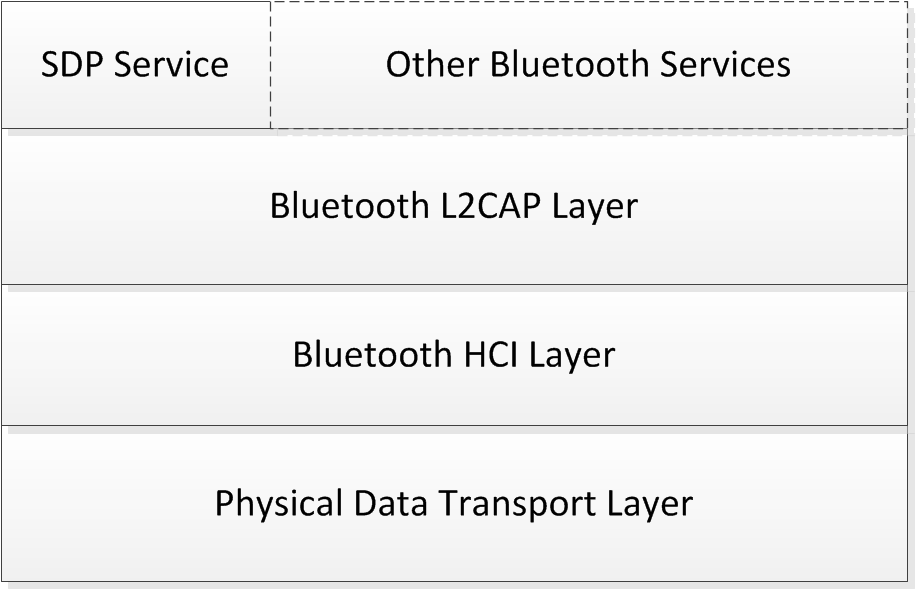
\includegraphics[width=80mm]{BluetoothStack.png}
	\rule{35em}{0.5pt}
	\caption[Diagram of a typical Bluetooth Stack]{Diagram of the basic components which form a typical Bluetooth Stack}
	\label{fig:btstack}
\end{figure}

As the usefulness of an abstract piece of software is inherently low without a suitable demonstration platform, a second component of the project will be to design, develop and prototype a functional and practical device which uses the created stack. It is proposed that this hardware component be in the form of a small \textit{"ExplorerBot"} robot, able to stream local sensor data wirelessly to a remote PC for real-time graphing purposes, and to allow for remote wireless control over a Bluetooth link to a consumer Bluetooth control device - such as a current generation Game Console controller (\textit{Wii} or \textit{Playstation 3}). If possible, these two functions should be combined to allow for multiple simultaneous connections, allowing for remote control at the same time as the sensor data is logged remotely.

% TODO - Figure of robot

With the combination of the software \emph{(the stack)} and hardware \emph{(the robot)} components of this project, the final design should offer a complete system and test platform which can be reproduced wholesale, modified to suit a particular application or used as a reference implementation for other projects.

\section{Design Goals}

The design goals of the project were split into two distinct parts, consisting of the software Bluetooth Stack implementation, and the physical robot hardware design. This separation of the testing platform hardware goals from those of the logical Bluetooth stack allowed for the clearest representation of the project as a whole.

\subsection{Software Goals}

For such a stack to be useful in an embedded environment, it must be able to conform to the restrictions such an environment imposes. Specifically, the completed stack must minimize its compiled and working set footprints, reduce or eliminate the need for dynamic memory allocation, and minimize its hardware dependencies to suit as wide a range of processors of differing capabilities as possible.

The design goals of the complete software stack were therefore set to:

\begin{itemize}
	\item Use as little RAM as possible
	\item Compile to as small a binary as is practical
	\item Offer a framework upon which services can be added to suit a particular application
	\item Provide asynchronous events to which the user application can respond to
	\item Allow for a variable number of simultaneous connections and logical channels to/from remote devices
	\item Have no requirement for dynamic memory allocation on the heap
	\item Allow for integration into an optional RTOS, but support stand-alone operation
	\item Be fully decoupled from the physical transport to the Bluetooth Adapter
	\item Be endian-correct regardless of native processor endianness
	\item Maintain a level of compatibility with Bluetooth Version 2.1 specification as maintained by the Bluetooth \textit{Special Interest Group} (SIG)
\end{itemize}

While at the point of the project's design and development a newer Bluetooth 3.0 version standard was available, a decision was made to implement the slightly older - and far more popular - version 2.1 of the Bluetooth specification. This decision was made due to the abundance of cheap Bluetooth 2.1 compatible hardware already of the market (and, conversely, the lack of cheap and widely available Bluetooth 3.0 hardware). In addition, the aim of the project was set to produce a \textit{compatible} rather than fully \textit{compliant} stack, due to the significantly increased development complexity of the latter for little additional benefit.

\subsection{Hardware Goals}

To make a useful, visual and functional testing platform, a decision was made to produce a small, battery powered robot. This robot would serve as both a testing platform for the completed stack to verify its correct operation in a real-world environment during development, and to function as a reference application of the completed stack.

In order to fully demonstrate the capabilities of the Bluetooth stack, the robot would have to include both locally initiated Bluetooth connections, as well as accept remotely initiated connections. In addition to this requirement, data would have to be both received and sent to and from a remote device to demonstrate full duplex communications.

A set of design goals was thus created for the robot:

\begin{itemize}
	\item Allow the user to initiate a connection to a remote device via the robot
	\item Accept incoming connections from remote Bluetooth devices, including some level of authentication
	\item Consume data received from remote Bluetooth device(s) via one or more Bluetooth services
	\item Produce data to be transmitted to remote Bluetooth device(s) via one or more Bluetooth services
	\item Visually indicate status and debug messages via a display mechanism, for debugging
	\item Allow for the robot to be remotely driven via a set of PWM controlled DC motors
\end{itemize}

% TODO

	\chapter{Existing Implementations}
\label{chp:existingimp}
\lhead{Chapter 2. \emph{Existing Implementations}}

Before work was started on the proposed software Bluetooth stack implementation, the existing field of Bluetooth stacks (both commercial and non-commercial) were evaluated to determine what capabilities are being offered.

\section{Classes of Existing Stacks}

During the course of the project background research into existing Bluetooth stacks, two distinct classes of stack were observed, each with distinct assumptions and capabilities:

\begin{itemize}
	\item \textbf{Operating System based Stacks}, which assumed that they would be run on top of a complex full-featured OS, containing a kernel- and user-space, virtualized memory, synchronisation primitives, etc.
	\item \textbf{Embedded Stacks}, which assumed no OS was present, but nevertheless made assumptions as to the environment's capabilities for dynamic memory allocation
\end{itemize}

These two classes of stacks show two possible approaches to an implementation; one, the designer may write a stack around an existing Operating System API, or two, the designer can assume a "freestanding" or "bare metal" environment, with either no, or only a minimal, RTOS being present.

\section{Existing Bluetooth Stacks}

Below the discovered existing Bluetooth stacks are listed in parametric form for each class of stack for ease of reference.

\subsection{Operating System Stacks}

\begin{table}[H]
	\begin{center}
		\begin{tabular}{ | l | l | l |}
			\hline
			\textbf{Stack Name}	& \textbf{Operating System}	& \textbf{Commercial} \\ \hline

			FreeBSD Stack		& FreeBSD	& No	\\ \hline
			Affix Stack			& Linux		& No	\\ \hline
			BlueZ Stack			& Linux		& No	\\ \hline
			Apple Stack			& MacOS		& Yes	\\ \hline
			BlueFritz! Stack	& Windows	& Yes	\\ \hline
			CSR Harmony Stack	& Windows	& Yes	\\ \hline
			FreeBT Stack 		& Windows	& No	\\ \hline
			Microsoft Stack		& Windows	& Yes	\\ \hline
			Toshiba Stack		& Windows	& Yes	\\ \hline
			Widcomm Stack		& Windows	& Yes	\\ \hline
		\end{tabular}
		\caption[Existing Operating System Bluetooth Stacks]{Parametric table of existing OS based Bluetooth stacks}
		\label{tab:osbtstacks}
	\end{center}
\end{table}

As expected, the vast majority of existing OS based Bluetooth stacks are targeted towards the Microsoft Windows operating system, due to its large market share. In almost all cases, the existing stacks were found to support a rich number of Bluetooth services, in both device and server roles. While the majority of the Bluetooth stacks on the market are commercialized (i.e. require payment or hardware purchase for a license to use them) there are still several free and open source stacks available for the various Linux and BSD kernels.

% TODO

\subsection{Embedded Stacks}

\begin{table}[H]
	\begin{center}
		\begin{tabular}{ | l | l |}
			\hline
			\textbf{Stack Name}	& \textbf{Commercial} \\ \hline

			BlueCode+ Stack		& Yes	\\ \hline
			BlueLet Stack		& Yes	\\ \hline
			BlueMagic Stack		& Yes	\\ \hline
			Bluetopia Stack		& Yes	\\ \hline
			BTStack Stack		& No	\\ \hline
			ClarinoxBlue Stack	& Yes	\\ \hline
			CSR Synergy Stack	& Yes	\\ \hline
			EtherMind Stack		& Yes	\\ \hline
			Jungo BTware Stack	& Yes	\\ \hline
			lwBT Stack			& No	\\ \hline
			Mecel Betula Stack	& Yes	\\ \hline
			Symbian OS Stack	& Yes	\\ \hline
		\end{tabular}
		\caption[Existing Embedded Bluetooth Stacks]{Parametric table of existing embedded Bluetooth stacks}
		\label{tab:embbtstacks}
	\end{center}
\end{table}

Contrasting with the OS based stacks discussed previously, almost all Bluetooth stacks aimed at the embedded market today were found to be exclusively commercialized, requiring large payments and license agreements before they could be integrated into existing designs. Of note in this area are the \textit{BTStack} and \textit{lwBT} embedded Bluetooth stacks, which were both found to be both free and open source, but suffered from the constraints of RTOS dependencies in the case of the former, and incompleteness in the case of the latter.

% TODO

	\chapter{Software Implementation}
\label{Chapter 3}
\lhead{Chapter 3. \emph{Software Implementation}}

% TODO

\section{Software Overview}

% TODO

\section{Design Restrictions}

% TODO

\section{Software Layers}

% TODO

\FloatBarrier
\subsection{Physical Transport}

% TODO

\FloatBarrier
\subsubsection{LUFA USB Stack}

% TODO

\FloatBarrier
\subsection{HCI Layer}

% TODO

\FloatBarrier
\subsection{L2CAP Layer}

% TODO

\FloatBarrier
\subsection{Bluetooth Services}

% TODO

\FloatBarrier
\subsubsection{SDP Service}

% TODO

\FloatBarrier
\subsubsection{HID Service}

% TODO

\FloatBarrier
\subsubsection{RFCOMM Service}

% TODO

\section{Integration into User Applications}

% TODO

\FloatBarrier
\subsection{Events and Callbacks}

% TODO

\FloatBarrier
\subsection{Management Functions}

% TODO
	\chapter{Hardware Implementation}
\label{Chapter 4}
\lhead{Chapter 4. \emph{Hardware Implementation}}

To help demonstrate the usefulness of the stack in a practical manner, a robot was designed and constructed. This robot, named the \emph{ExplorerBot}, was then used to give a practical reference implementation of a full project utilizing the custom embedded Bluetooth stack in a real-world environment.

\section{Hardware Overview}

The completed robot design for the project contains many useful capabilties for both mobility and exploration. Built on top of a pre-fabricated (including raw DC motors and gearing) "Tank" style hobby robot base, the \emph{ExplorerBot} robot implements the following features:

\begin{itemize}
	\item Primary switch-mode based 5V power supply
	\item Secondary LDO based 3.3V power supply for attached sensors
	\item 2x16 Alphanumeric LCD Screen for feedback to the user
	\item Two momentary pushbuttons for user control
	\item One RGB status LED for basic status feedback
	\item Dual PWM motor control system, with variable speed and direction of DC motors
	\item Level converted I\textsuperscript{2}C bus for the attached sensor(s)
	\item Support for the Atmel \textit{Inertial One} and \textit{Pressure One} sensor boards
	\item High intensity LED based headlights for frontal illumination
	\item Piezo speaker for audio feedback and "horn" like functionality
	\item Atmel \textit{AT90USB1287} 8-Bit Microcontroller
	\item External 128KB SRAM for temporary storage of packets to and from the Bluetooth adapter
\end{itemize}

The complete robot design was created in the \textit{Altium Designer} software, including both the schematic design and board routing. Surface mount components were chosen where possible to reduce the board space required, and two board layers used as this proved to offer the lowest cost/time ratio. The final board design measured 10cm x 15cm, however much of this board space is relatively unused; with optimization, this board space could be reduced considerably.

To get the best results in the construction of the robot, the boards were manufactured commercially. This process ensured the manufactured board's quality while also provided solder mask and silkscreen to reduce the potential for error in the robot's construction.

\section{Hardware Modules}

In the section, the various hardware components of the constructed robot are detailed at the block level. Figure \ref{fig:robotblockhw} below illustrates how the various hardware blocks that comprise the robot connect together to make the final design.

\vspace{1em}

\begin{figure}[H]
	\centering
		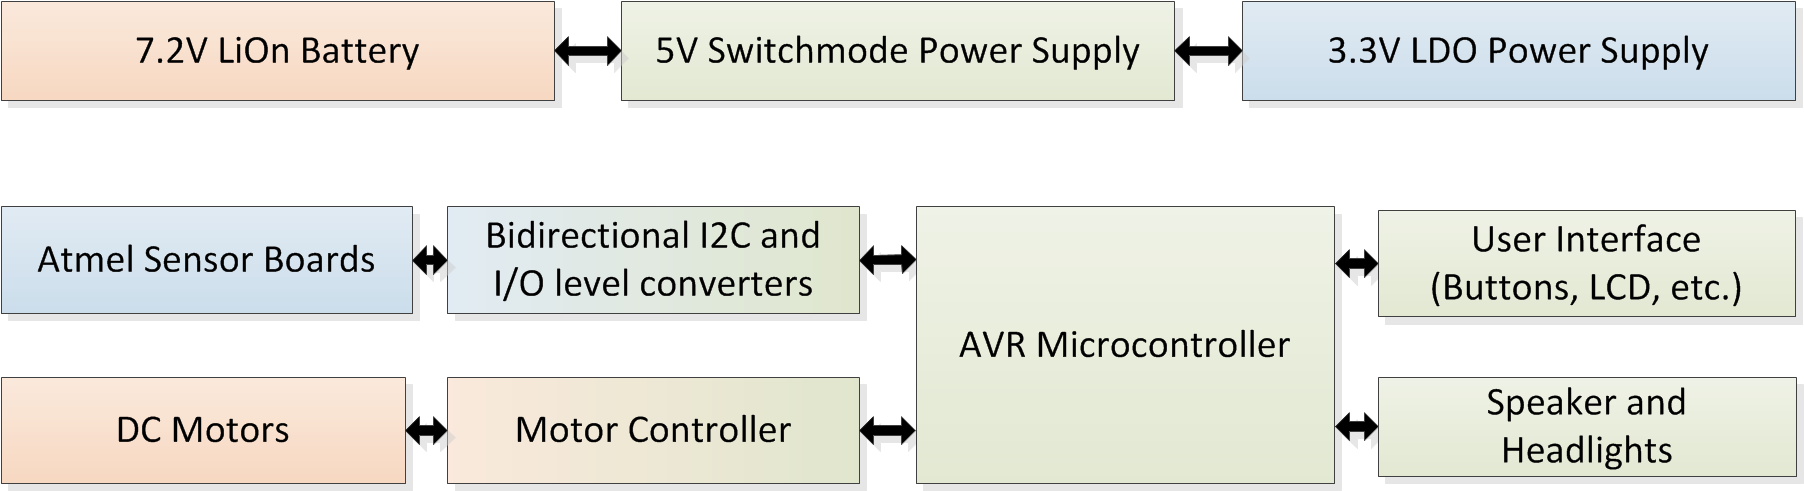
\includegraphics[width=140mm]{./Figures/BlockDiagram.png}
	\rule{35em}{0.5pt}
	\caption[Hardware Block Diagram]{Robot Hardware Block Diagram}
	\label{fig:robotblockhw}
\end{figure}

\subsection{Microprocessor}

Due to the author's familiarity with the Atmel line of \textit{AVR} branded microcontrollers, one of the avaliable models in this line-up was chosen to serve in the robot as the main processor, the AT90USB1287. This 8-bit microcontroller contains 128KB of non-voltatile FLASH memory for program storage, 4KB of non-voltatile EEPROM for user application parameter storage and 8KB of internal SRAM for scratch memory. A 16MHz clock (provided by an external crystal) was selected for the design as this offered the fastest possible speed the chip was capable of, while still allowing the hardware USB host controller inside the chip to function normally. As a trade-off, this higher clock speed put a constraint on the main logic level voltage; at 16MHz, the AVR microcontroller required 5V to be within the datasheet's specifications.

As the AT90USB1287 and associated USB components are difficult to source in single quantities at reasonable prices, the use of a commercial breakout module containing this chip was selected instead: the \textit{Micropendous-A} board (see Figure \ref{fig:micropendous}). This board contains the surface mount AVR microcontroller and associated USB components, along with an external 128KB SRAM chip attached to the AVR's external memory bus interface. As the Bluetooth stack required a large temporary buffer for incoming fragments, the selection of this board proved ideal for the intended purpose.

\begin{figure}[h]
	\centering
		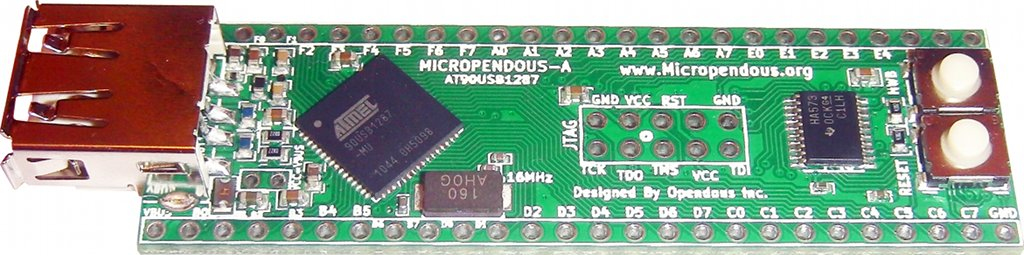
\includegraphics[width=100mm]{./Figures/MicropendousA.jpg}
	\rule{35em}{0.5pt}
	\caption[Micropendous-A Board]{The Micropendous-A Board (Image courtesy \textit{Opendous Inc.})}
	\label{fig:micropendous}
\end{figure}

\subsection{Primary Power Supply}

As the vast majority of the robot's hardware operated at a fixed 5V level, a power supply was required to reduce the Lithium Ion battery's raw 7.2V (nominal) voltage down to the 5V level needed to power the various components. Due to the use of battery power in the project, reducing power consumption where possible was a large concern; thus, a switchmode design was chosen for maximum voltage conversion efficiency. A conventional linear regulator was considered for the design, but rejected due to the prohibitably large amount of power this would waste (approximately .45W, assuming an average 200mA operating current).

The regulator selected for the project was the M2595S-5.0, a fixed-function switchmode regulator capable of outputing a fixed 5V rail at loads of up to 3A. While the robot design would not consume even a fifth of this power, the overhead in the specifications ensured that the power supply would remain robust and the output within the tollerances of the system components regardless of the load demanded. The exact schematic used in the final robot power supply design (see Figure \ref{fig:mainpowersupply}) was taken from the regulator component's datasheet to ensure correct operation.

\begin{figure}[h]
	\centering
		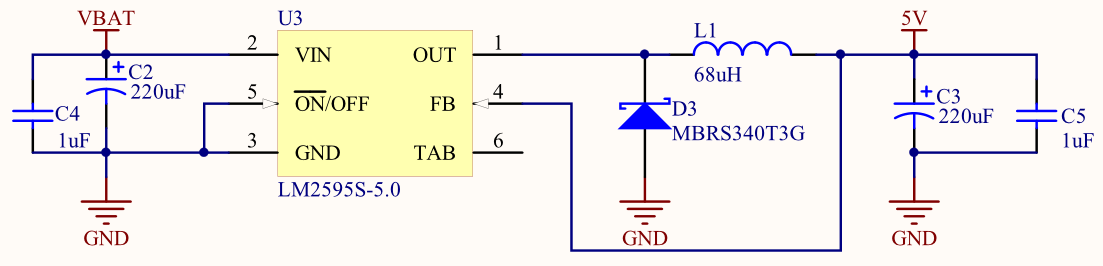
\includegraphics[width=150mm]{./Figures/MainPowerSupply.png}
	\rule{35em}{0.5pt}
	\caption[Main Power Supply Schematic]{Schematic of the robot's main 5V switchmode power supply.}
	\label{fig:mainpowersupply}
\end{figure}

\subsection{User Interface}

For interaction with the user, the robot contains several components, detailed below.

\subsubsection{RGB Status LED}

For primary status indication, a surface mount RGB LED indicates the current status of the robot. Due to a lack of free PWM channels on the AVR microcontroller, the three LED subcomponents are wired directly to standard GPIO ports. While this prevents PWM fading from producing a many-bit custom colour from the LED, a three bit colour space is possible giving a total of 7 possible colours (and no colour when all the LED subcomponents are turned off). For the purposes of the created robot, this is in practice more than enough for basic status indication.

To achieve a somewhat uniform brightness, the three LEDs were adjusted with current limiting resistors to consume an equal amount of current (approx. 5mA) despite differing forward voltages. As the RGB status LED shares the same I/O pins as the microcontroller's JTAG port for programmign and debugging, the RGB LED's common annode was connected via a removable wire link to ensure that it could be taken out-of-circuit if it proved to intefere with the external hardware debugger during development.

\subsubsection{LCD Display}

For situations where more information needs to be communicated to the user than is possible via the RGB status LED, a 16x2 Alphanumeric LCD display - compatible with the well known Hitatchi HD44780 chipset - was added to the design. Due to the limited number of GPIO pins avaliable on the microcontroller, the LCD was wired in 4-bit mode, with the lower 4 data pins on the LCD being wired directly to ground. While this doubled the time required to send a byte to the LCD (as bytes then need to be split into a pair of 4-bit nibbles) the high speed of the processor meant that in practice this had little or no effect to the overall speed of the system.

The LCD backlight was wired through a driver transistor to a spare PWM channel on the AVR microcontroller, allowing for 8-bit PWM brightness control to reduce power consumption of the backlight when not in use.

\subsubsection{Buttons}

A pair of standard PCB round buttons were added to the design, for user input. These buttons were wired directly to the microcontroller's GPIO pins; internal pull-up resistors in the microcontroller takes care of maintaining a defined logic level on the pins when the buttons are released, while software handles the debouncing of the button signals.

\subsection{Headlights}

To provide illumination of the area immediately ahead of the robot, a pair of high intensity white LEDs were added to the schematic, connected to a single common driver transistor and driven by a GPIO pin of the microcontroller. To ensure maximum illumination, the LEDs were driven at just under their full 20mA rating when turned on. These "headlights" were then mounted on the front of the robot chassis.

\subsection{Speaker}

A small PCB Piezo speaker was added to the robot, in order to provide both audio feedback for important events (such as Bluetooth connections and disconnections) as well as to act as a miniature horn to attract the attention of any organic obstacles to encourage then to move away from the robot's line of motion. Rather than mounting the speaker directly onto the PCB, it was determined that a better location was in between the two frontal headlight LEDs, with the speaker then connected back to the PCB via flyleads. This arrangement made the directional speaker point in the orientation most suited to a car horn, i.e. towards the front of the robot (see Figure \ref{fig:speakermouting}).

\begin{figure}[h]
	\centering
		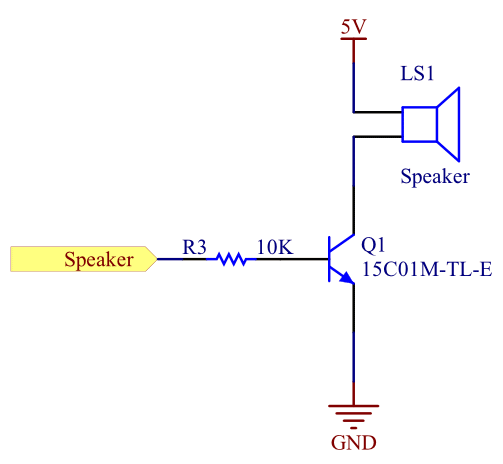
\includegraphics[width=55mm]{./Figures/SpeakerSchematic.png}
		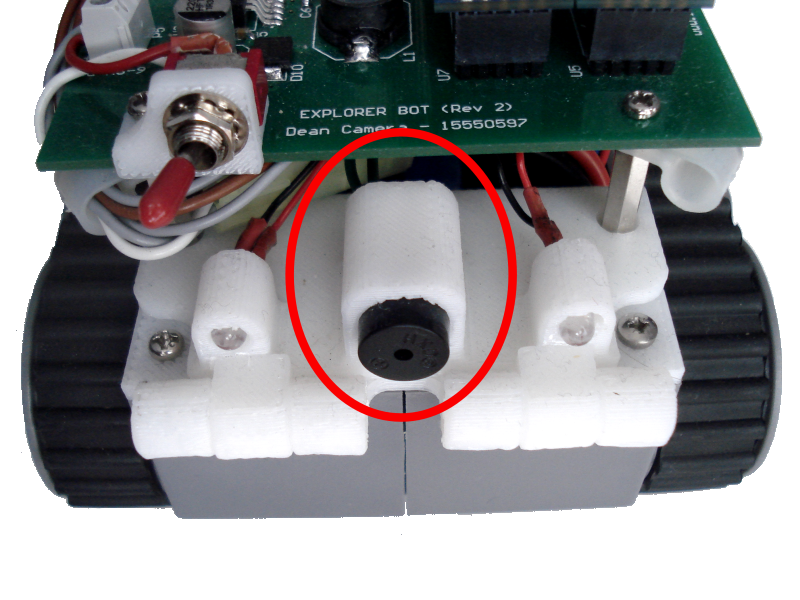
\includegraphics[width=60mm]{./Figures/RobotFront.png}
	\rule{35em}{0.5pt}
	\caption[Speaker Schematic and Mouting Photo]{Schematic of the robot's piezo speaker (\textit{left}) and photo showing the mouting in the robot prototype (\textit{right}).}
	\label{fig:robotspeaker}
\end{figure}

To drive the speaker, a standard NPN transistor was employed to provide sufficient current, driven from an 8-bit PWM timer output GPIO pin of the AVR microcontroller.

\subsection{Motor Controller}

% TODO

\subsection{Sensors}

To provide a measure of feedback from the robot, a number of sensors were added to the design. These sensors, when attached, would allow for the robot's environment to be logged and (potentially) reacted to.

\subsubsection{Sensor Power Supply}

While the main system logic and user interface components run from the main switch-mode 5V power supply, the sensor boards were required to run at a fixed 3.3V level, without the possibility of conversion to suit the higher rail voltage.

For this reason, and to reduce the amount of noise on the sensor power supply for maximum precision, a desision was made to add a secondary power supply, running from the 5V rail, to step down the voltage to the 3.3V required by the sensor boards. For best results, an ADP3308 Low Dropout (LDO) style regular was used as this provided both low output rail noise and minimal wasted power.

\subsubsection{Level Converters}

Due to the differing bus voltages between the sensor boards (3.3V) and the main processor (5V), level conversion of the I\textsuperscript{2}C bus and sensor interrupt/control lines was required. While only a unidirectional buffer was strictly needed for each of the sensor interrupt/control lines, it was decided to use a bidirectional converter to ease the board routing.

Initially, only an ADG3308 8-channel Bidirectional Level Converter IC was used, for both the sensor interrupt/control lines, as well as the I\textsuperscript{2}C bus. However, after further analysis it was discovered that the level translater would not meet the timing requirements of the I\textsuperscript{2}C bus, neccesitating the addition of a secondary dedicated Texas Instruments PCA9306 fixed function I\textsuperscript{2}C bus level converter IC in the second revision of the board. As a bonus, the use of the later chip allowed the I\textsuperscript{2}C bus to be driven at the "Fast" I\textsuperscript{2}C speed of 200KHz for minimal latency and maximum throughput.

Unusually, the ADG3308 level converter IC required that its enable pin (located on the low voltage side of the translator) be connected to the higher logic level for the chip to become active (see \ref{fig:ADG3308schematic}). This odd placement of the enable pin resulted in a non-optimal breaking of the ground plane underneath the chip to accomodate the required route, as the space between the chip package pins on the top layer was used to carry the 3.3V power bus to the sensor boards (see Figure \ref{fig:ADG3308routing}).

\begin{figure}[h]
	\centering
		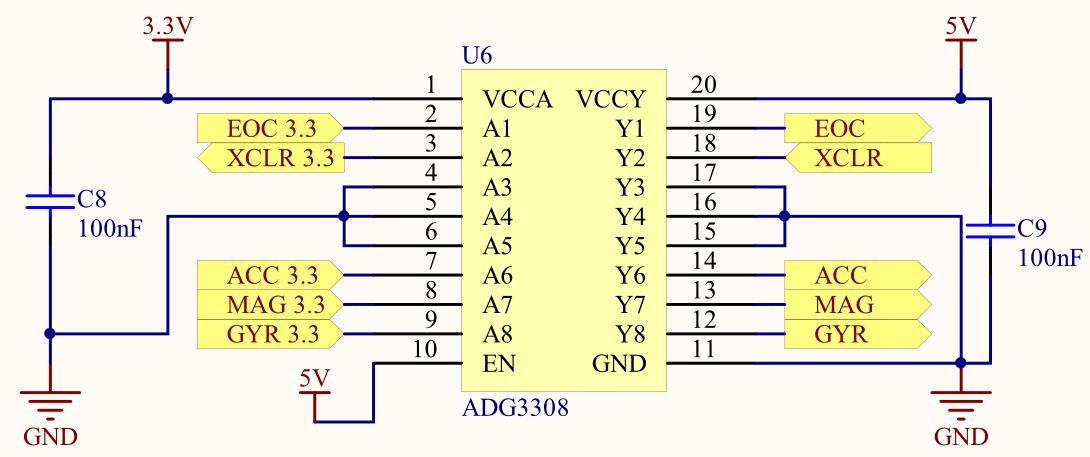
\includegraphics[width=120mm]{./Figures/LevelTranslatorSchematic.png}
	\rule{35em}{0.5pt}
	\caption[Bidirectional Level Translator Schematic]{Schematic of the ADG3308, showing the unusual placement of the enable pin.}
	\label{fig:ADG3308schematic}
\end{figure}

The board routing complexity was reduced slightly by swapping the functions of the PCA9306 bus level translatator's SDA and SCL pins (see Figure \ref{fig:PCA9306schematic}) on both sides of the IC; this modification (allowable as indicated in the device's datasheet) prevented the need to introduce additional board vias and longer trace routes.

\begin{figure}[h]
	\centering
		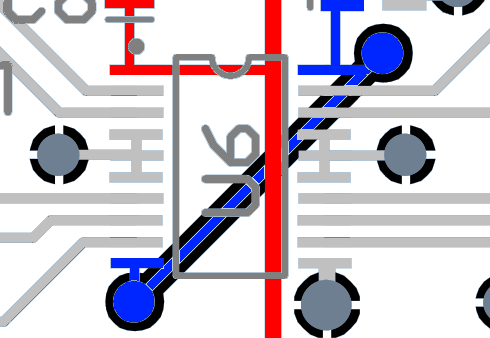
\includegraphics[width=50mm]{./Figures/LevelConverterRouting.png}
	\rule{35em}{0.5pt}
	\caption[Bidirectional Level Translator Routing]{Routing of the ADG3308, showing the 3.3V bus (red) and 5V enable (blue) routes.}
	\label{fig:PCA9306routing}
\end{figure}

\subsubsection{Atmel Sensor Boards}

By designing the robot around a pair of commercially available Atmel sensor boards for environmental feedback, the design of the robot was considerably simplified and the total unit cost lowered. The \textit{Atmel Pressure One} board contains a Bosch BMP085 Pressure Sensor IC for air pressure sensing, while the Atmel \textit{Inertial One} contains a 3-Axis ITG3200 Gyroscope, 3-Axis BMA150 Accelerometer and 3-Axis AK8975 Compass IC (see Figure \ref{fig:atmelsensorboards}). As several of the sensors also contain a digital temperature sensor in addition to the primary sensor (for calibration and stability feedback) this functionality was also used by the robot to measure the environmental temperature in real time.

Each sensor IC is driven by the main microcontroller of the robot over the level converted I\textsuperscript{2}C bus and one or more digital interrupt/control lines. The Atmel sensor board modules all use an identical form factor, with one standard .1" 2x5 female header located at one end of the board reserved for the mounted sensor's digital I/O pins, and another located at the opposite end of the board reserved for analogue sensor pinouts. As none of the sensor boards used contained analogue sensor outputs, the second female header consisted only of non-connected pins, and a matching male header was placed on the board for mechanical stability only.

\begin{figure}[h]
	\centering
		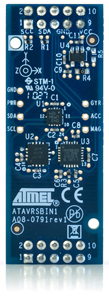
\includegraphics[height=70mm]{./Figures/Inertial1.jpg}
		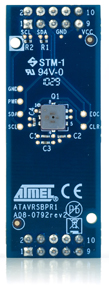
\includegraphics[height=70mm]{./Figures/Pressure1.jpg}
	\rule{35em}{0.5pt}
	\caption[Atmel Sensor Boards]{The Atmel \emph{Inertial One} (left) and \emph{Pressure One} (Right) Sensor Boards (Image courtesy \textit{Atmel Corp.})}
	\label{fig:atmelsensorboards}
\end{figure}


	\chapter{Robot Firmware Implementation}
\label{Chapter 5}
\lhead{Chapter 5. \emph{Robot Firmware Implementation}}

With the creation of the software embedded Bluetooth stack and the \textit{ExplorerBot} test robot platform hardware, it was neccesary to integrate these two components into a functional prototype. By using the Bluetooth stack in a real-world, practical application while it was being developed, the quality, effectiveness and completeness of the stack could be evaluated.

\section{Build Dependencies}

To match the Bluetooth stack, each module was written in the C language, and targeted at the free open source AVR-GCC compiler and avr-libc library. A standard \textit{makefile} included with the firmware allows for command line control over the building of the project files into a set of binaries which can then be programmed into the target microcontroller for use via the command \texttt{make all}. The following tools are required to build the firmware under Windows:

\begin{itemize}
	\item The \textbf{WinAVR 20100101} release download, or Windows binaries of the \textbf{GNU Shell Utilities}
	\item The latest \textbf{AVR Toolchain} release from Atmel (Included with Atmel's free \textit{AVRStudio 5} software)
\end{itemize}

Under Debian Linux environments, the following packages are required:

\begin{itemize}
	\item \textbf{gcc-avr} 
	\item \textbf{binutils-avr}
	\item \textbf{avr-libc}
	\item \textbf{avrdude}
\end{itemize}

Which can be installed via the command prompt using the command \texttt{sudo apt-get install gcc-avr binutils-avr avr-libc avrdude}.

\section{Firmware Overview}

The completed firmware of the \textit{ExplorerBot} prototype was developed in a modular manner, to match the corresponding hardware components. This top-down methodology ensured that each portion of the firmware could be mocked up, tested and integrated as needed. Additionally, seperating out the firmware components into logical modules gave the final firmware a level of flexibility which should allow for easy modification to suit any hardware changes made to those of the prototype. The completed set of modules (see Figure \ref{fig:robotblockfw}) served as the complete firmware for the robot.

\begin{figure}[H]
	\vspace{1em}
	\centering
		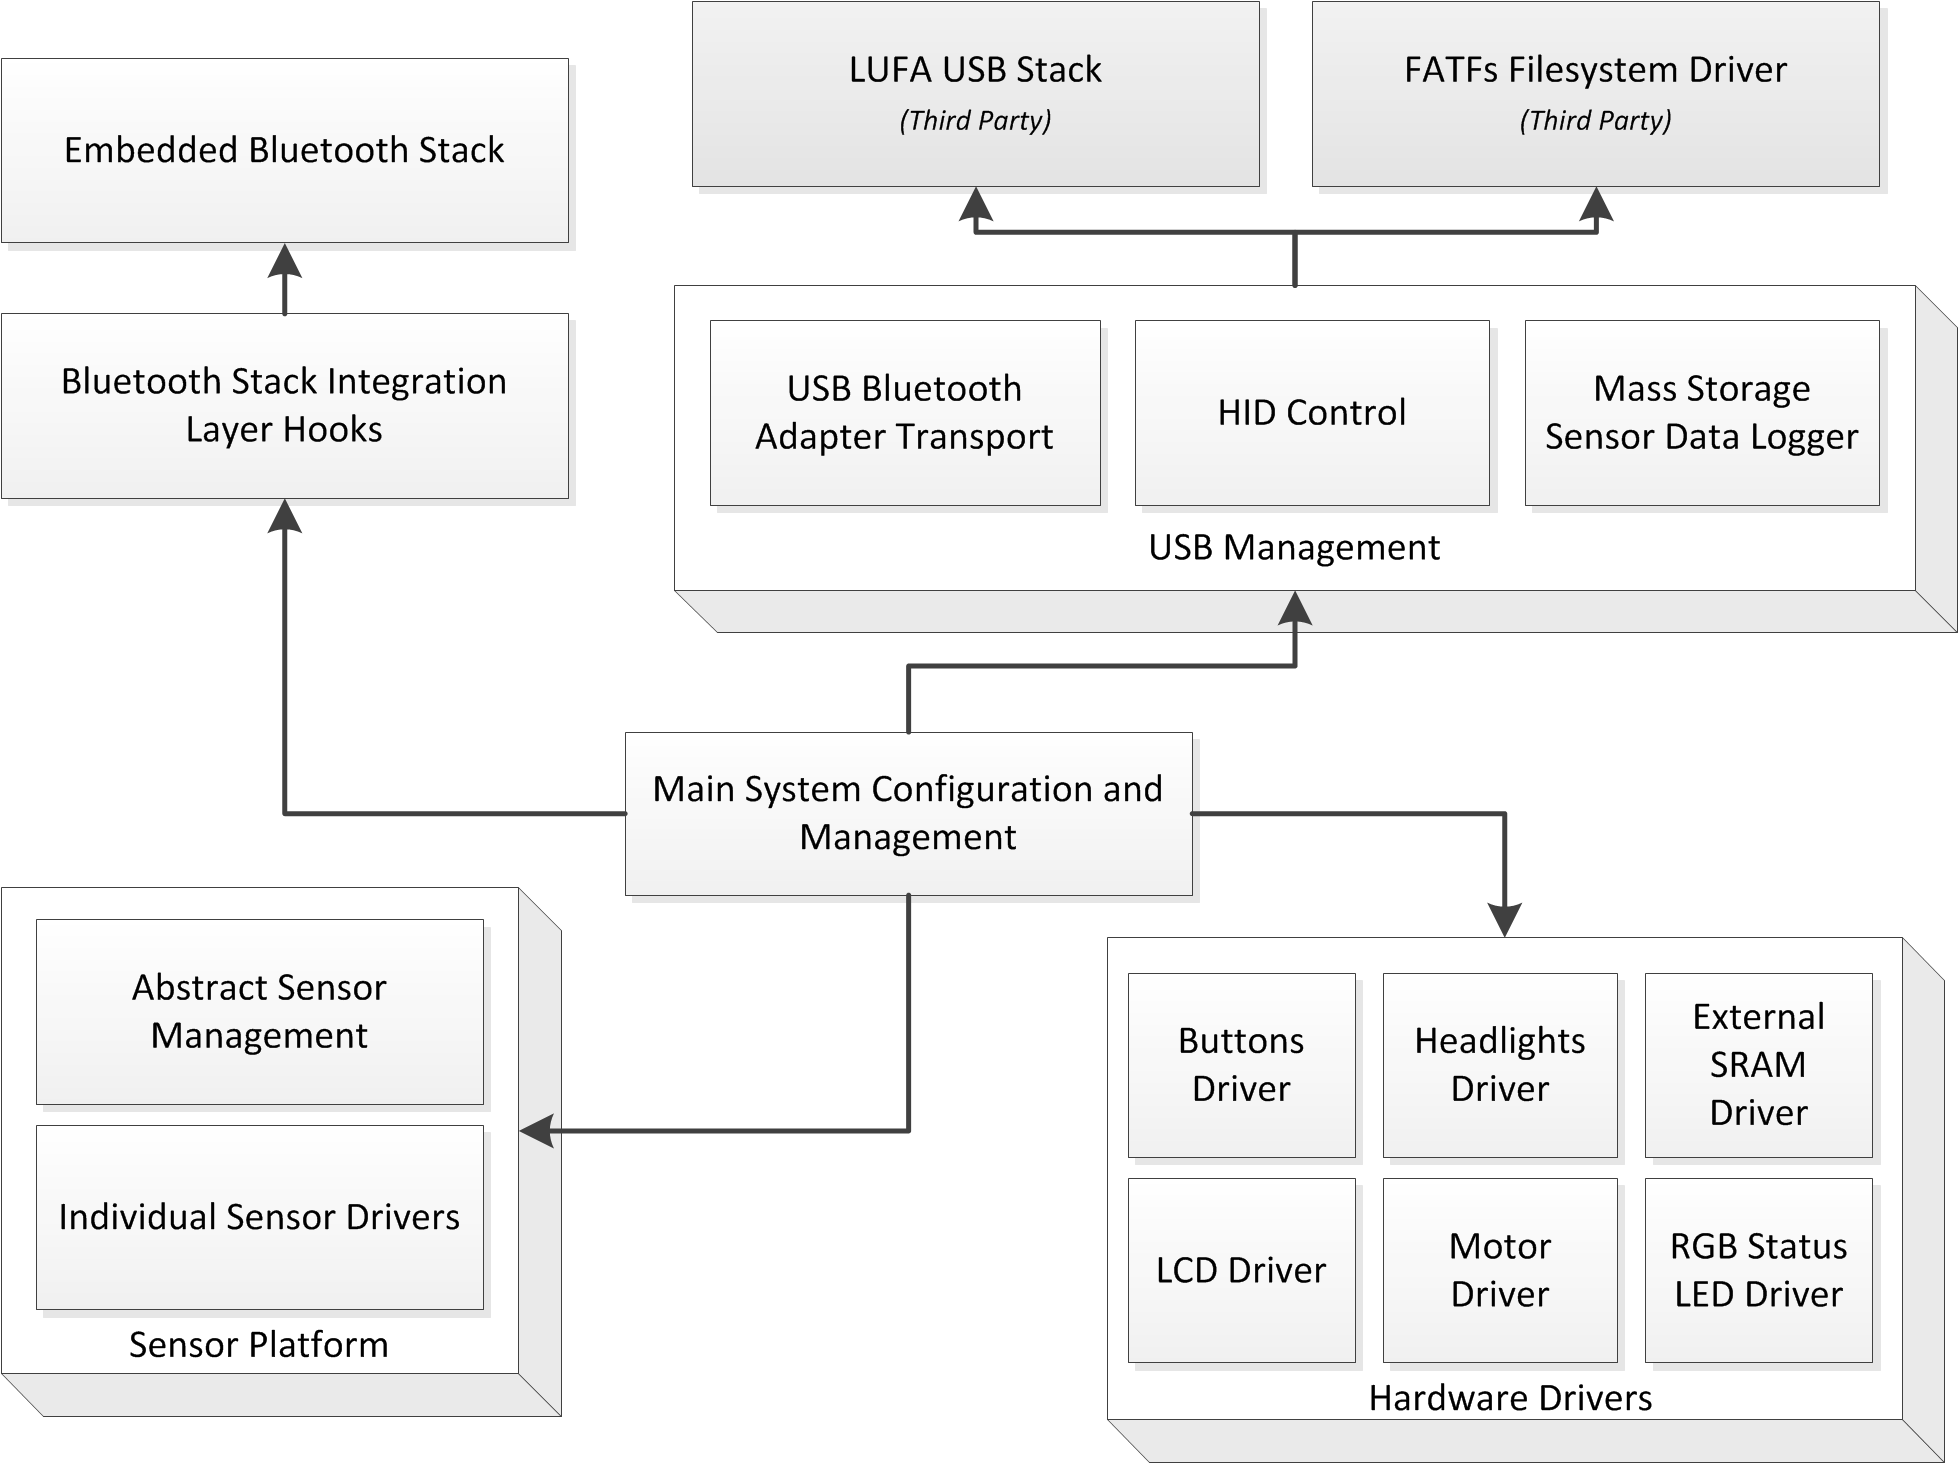
\includegraphics[width=140mm]{FirmwareBlockDiagram.png}
	\rule{35em}{0.5pt}
	\caption[Firmware Block Diagram]{Robot Firmware Block Diagram}
	\label{fig:robotblockfw}
\end{figure}

\section{Firmware Modules}

In this section, each of the robot firmware's main software modules are listed and described in additional detail so that the overall design and implementation of the firmware can be further understood.

\FloatBarrier
\subsection{Main System Control and Configuration}

% TODO

\FloatBarrier
\subsection{Hardware Drivers}

% TODO

\FloatBarrier
\subsection{Sensor Platform}

% TODO

\FloatBarrier
\subsubsection{Abstract Sensor Management}

% TODO

\FloatBarrier
\subsubsection{Individual Sensor Drivers}

% TODO

\FloatBarrier
\subsection{USB Management}

% TODO

\FloatBarrier
\subsubsection{Bluetooth Adapters}

% TODO

\FloatBarrier
\subsubsection{HID Devices}

% TODO

\FloatBarrier
\subsubsection{Mass Storage Devices}

% TODO

\FloatBarrier
\subsection{Bluetooth Management}

% TODO

\FloatBarrier
\subsubsection{Stack Integration Layer}

% TODO

\FloatBarrier
\subsubsection{Bluetooth Stack}

% TODO

\FloatBarrier
\subsection{Third Party Modules}

% TODO

\FloatBarrier
\subsubsection{LUFA}

% TODO

\FloatBarrier
\subsubsection{FatFS}

% TODO

	\chapter{Project Discussion}
\label{Chapter 6}
\lhead{Chapter 6. \emph{Project Discussion}}

% TODO


	\chapter{Project Discussion}
\label{chp:discussion}
\lhead{Chapter 7. \emph{Project Discussion}}

% TODO

	
%% ----------------------------------------------------------------
\setstretch{1.5}  % Set the line spacing to 1.5, this makes the following tables easier to read
\clearpage  % Start a new page
\lhead{\emph{Abbreviations}}  % Set the left side page header to "Abbreviations"
\listofsymbols{ll}  % Include a list of Abbreviations (a table of two columns)
{
	\textbf{AVR} & This isn't an acronym. Officially, at least. \\
	\textbf{GPIO} & \textbf{G}eneral \textbf{P}urpose \textbf{I/O} \\
	\textbf{HCI} & Bluetooth \textbf{H}ost \textbf{C}ontroller \textbf{I}nterface \\
	\textbf{HID} & \textbf{H}uman \textbf{I}nterface \textbf{D}evice \\
	\textbf{IC} & \textbf{I}ntergrated \textbf{C}ircuit \\
	\textbf{I\textsuperscript{2}C} & \textbf{I}nter \textbf{I}ntegrated \textbf{C}ircuit Bus \\
	\textbf{L2CAP} & Bluetooth \textbf{L}ogical \textbf{L}ink \textbf{C}ontrol and \textbf{A}daption \textbf{P}rotocol \\
	\textbf{LED} & \textbf{L}ight \textbf{E}mitting \textbf{D}iode \\
	\textbf{LUFA} & \textbf{L}ightweight \textbf{U}SB \textbf{F}ramework for \textbf{A}VRs \\
	\textbf{PCB} & \textbf{P}rinted \textbf{C}ircuit \textbf{B}oard \\
	\textbf{PWM} & \textbf{P}ulse \textbf{W}idth \textbf{M}odulation \\
	\textbf{RTOS} & \textbf{R}eal \textbf{T}ime \textbf{O}perating \textbf{S}ystem \\
	\textbf{SDP} & Bluetooth \textbf{S}ervice \textbf{D}iscovery \textbf{P}rotocol \\
}
%% ----------------------------------------------------------------
\addtocontents{toc}{\vspace{1em}} % Add a gap in the Contents, for aesthetics
\appendix % Cue to tell LaTeX that the following 'chapters' are Appendices

	\chapter{Schematics}
\label{Appendix A}
\lhead{Appendix A. \emph{ExplorerBot Robot Schematics}}

\section{Robot Schematics}

The following pages illustrate the complete schematics of the \emph{ExplorerBot} robot hardware created to demonstrate a practical application of the Bluetooth stack.

\includepdf[pages=4, landscape, offset=80 -70]{./Appendices/Schematics.pdf}
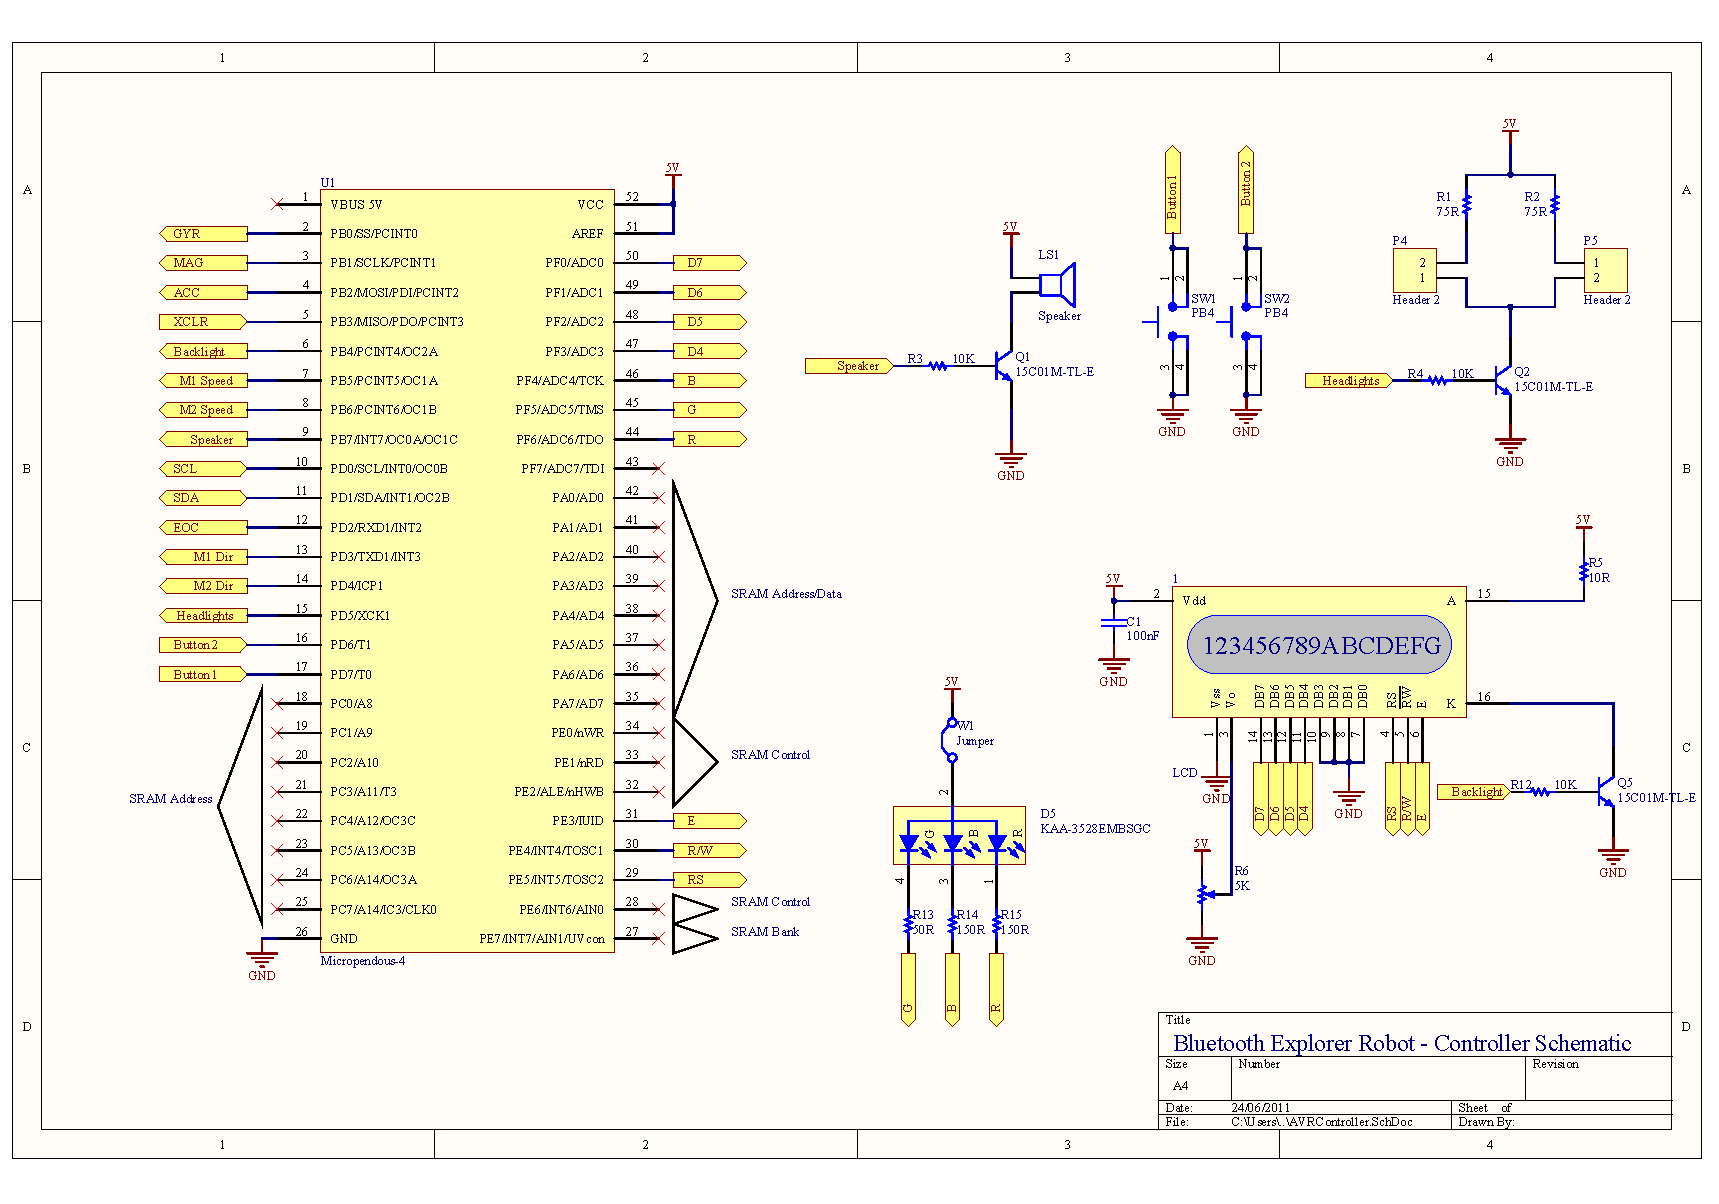
\includepdf[pages={1-3}, landscape, offset=80 -70]{./Appendices/Schematics.pdf}
\includepdf[pages=5, landscape, offset=80 -70]{./Appendices/Schematics.pdf}
	\chapter{Stack API Overview}
\label{app:stackapi}
\lhead{Appendix C. \emph{Stack API Overview}}

% TODO
	\chapter{Robot User Guide}
\label{app:robotuserguide}
\lhead{Appendix \ref{app:robotuserguide}. \emph{Robot User Guide}}

% TODO

\section{Power Requirements}

% TODO

\section{Supported USB Devices}

% TODO

\subsection{HID Class Devices}

% TODO

\subsection{Mass Storage Class Devices}

% TODO

\subsection{Bluetooth Adapter Devices}

% TODO

\section{Supported Bluetooth Services}

% TODO

\subsection{HID Service}

% TODO

\subsection{RFCOMM Service}

% TODO
	\chapter{Host Application User Guide}
\label{Appendix D}
\lhead{Appendix D. \emph{Host Application User Guide}}

\begin{center}
	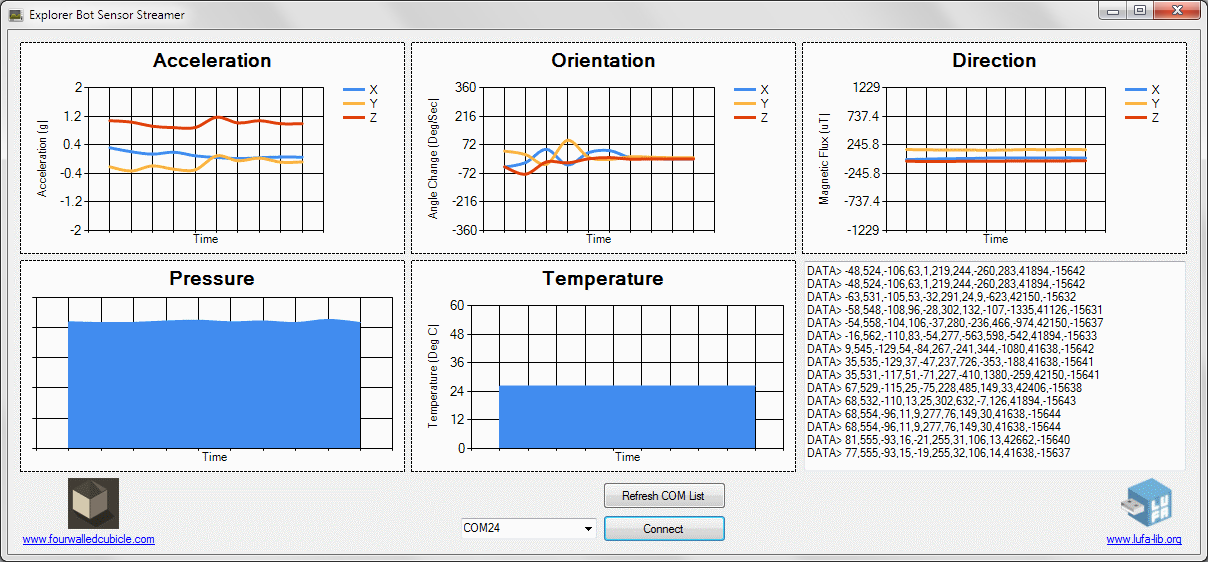
\includegraphics[height=70mm]{./Figures/SensorDataApp.png}
\end{center}

% TODO

\section{System Requirements}

% TODO

\section{Connecting to the Robot}

% TODO

	
\addtocontents{toc}{\vspace{2em}}  % Add a gap in the Contents, for aesthetics
\backmatter
%% ----------------------------------------------------------------
\label{Bibliography}
\lhead{\emph{Bibliography}}  % Change the left side page header to "Bibliography"
\bibliographystyle{unsrtnat}  % Use the "unsrtnat" BibTeX style for formatting the Bibliography
\bibliography{Bibliography}  % The references (bibliography) information are stored in the file named "Bibliography.bib"
\end{document}  % The End
%% ----------------------------------------------------------------
